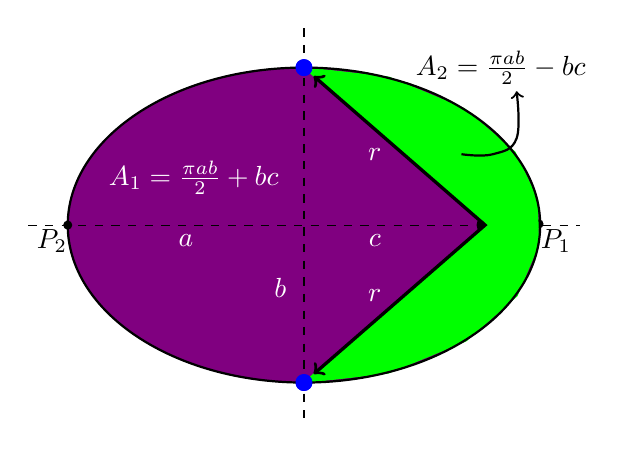
\begin{tikzpicture}
\draw  [fill, violet](-1,1) ellipse (3 and 2);

\draw [dashed](-4.5,1) -- (2.5,1);
\draw  [dashed](-1,3.5) -- (-1,-1.5);
\draw  [fill](1.3,1) node (v2) {} circle (0.1);
\node at (1.3,0.6) {O};
\draw  [fill](-4,1) circle (0.05);
\draw [fill] (1.9855,1.0145) node (v4) {} circle (0.05);
\node at (-4.2,0.8) {$P_2$};
\node at (2.2,0.8) {$P_1$};


\draw  [fill, green]plot[smooth, tension=0] coordinates {(1.2859,1.0479) (-1,3) (0.08,2.8783) (1.0362,2.4783) (1.6812,1.9261) (1.9653,1.3246) (1.9782,0.7464) (1.7061,0.1016) (1.058,-0.471) (0.0685,-0.8796) (-1,-1) (1.3018,1.003)};
\draw  [fill, blue] (-1,3) node (v1) {} circle (0.1);
\draw  [fill, blue](-1,-1) node (v3) {} circle (0.1);
\draw [<->, very thick] (v1) -- (v2.center) -- (v3);
\draw  [thick](-1,1) ellipse (3 and 2);
\node at (-2.4,1.6) [white] {$A_1=\frac{\pi a b}{2}+bc$};
\node at (1.5,3) {$A_2=\frac{\pi a b}{2}-bc$};
\draw  [->, thick]plot[smooth, tension=.7] coordinates {(1,1.9) (1.4,1.9) (1.7,2.1) (1.7,2.7)};
\node at (-0.1,1.9) [white] {$r$};
\node at (-0.1,0.1) [white] {$r$};
\node at (-0.1,0.8) [white] {$c$};
\node at (-1.3,0.2) [white] {$b$};
\node at (-2.5,0.8) [white] {$a$};
\draw  [fill, blue] (-1,3) node (v1) {} circle (0.1);
\draw  [fill, blue](-1,-1) node (v3) {} circle (0.1);
\end{tikzpicture}